\documentclass[11pt, oneside]{article}   	% use "amsart" instead of "article" for AMSLaTeX format
\usepackage{geometry}                		% See geometry.pdf to learn the layout options. There are lots.
\geometry{letterpaper}                   		% ... or a4paper or a5paper or ... 
%\geometry{landscape}                		% Activate for rotated page geometry
%\usepackage[parfill]{parskip}    		% Activate to begin paragraphs with an empty line rather than an indent
\usepackage{graphicx}				% Use pdf, png, jpg, or eps§ with pdflatex; use eps in DVI mode
								% TeX will automatically convert eps --> pdf in pdflatex		
\usepackage{amssymb}
\usepackage{paralist}
\usepackage{listings}
\usepackage{hyperref}
\lstset{breaklines = true}
\hypersetup{colorlinks=true,
    linkcolor=blue,
    citecolor=blue,
    filecolor=blue,
    urlcolor=black,
    unicode=false}

\usepackage{fancyhdr}
\fancyhead[L]{\today\ }
\fancyhead[C]{SE 3XA3 Test Plan}
\fancyhead[R]{Genzter}
\pagestyle{fancy}

\usepackage{float}


%SetFonts

%SetFonts


\title{Test Plan: Revision 1}
\author{Group 2 - Genzter \\
		\\ Binu, Amit - binua - 400023175
		\\ Bengezi, Mohamed - bengezim - 400021279
		\\ Samarasinghe, Sachin - samarya - 001430998
		\\Professor: Dr. Bokhari
		\\ Lab: L01}

\begin{document}

\maketitle
\newpage
\tableofcontents
\listoffigures
\listoftables

\newpage
\section{Revision History}

\begin{table}[h]
\begin{center}
\begin{tabular}{ | c | c | c | c | }
\hline
 Date & Version & Description & Author \\ 
\hline
 23/OCT/17 & 0.0 & Created Test Plan & Mohamed Bengezi, Amit Binu, Sachin Samarasinghe \\  
\hline
 27/OCT/17 & 0.0 & Updated Test Plan & Mohamed Bengezi \\  
\hline
 21/NOV/17 & 1.0 & Updated for Revision 1 & Mohamed Bengezi \\
\hline 
 06/DEC/17 & 1.0 & Changed some tests to automated & Mohamed Bengezi \\ 
\hline 
\end{tabular}
\end{center}
\caption{Revision History}
\end{table}

**Please note that all additions and modificiations are in  \textcolor{blue}{blue}



\newpage
% 
\section{Introduction}
\subsection{Purpose}
\textcolor{blue}{The purpose of this document is to document the testing plans and procedures that the system will undergo. It will outline the general definition/purpose of each type of test, and how those tests will be implemented with regards to this project.} The goal of this project is to create a viable set of schedules for the user based on the inputted courses. All corresponding core's, labs, and tutorials must be included in each timetable. \\
The automated testing shall include unit testing performed by the Mocha framework for javascript. Functional testing shall consist of input testing, along with conflict tests, and perfect input tests. Structural testing shall include performance tests, such as a large number of courses as input, as well as dataset traversal tests. Fault and Mutation testing will occur throughout development. Manual testing, such as static testing, shall be done primarily by group code walkthrough's \& inspections, in order to check syntax and logic, and gain a better understanding of the program code as a whole. Dynamic testing shall include using a number of predetermined schedules from various programs, and using the courses on each schedule as input, and determining that each necessary core, lab, and tutorial are listed in the generated timetable. 

\subsection{Definitions}

\begin{itemize}

\item \textcolor{blue}{Static Testing: Testing that does not involve program execution. This includes syntax checking, document and code walkthroughs/inspections, correctness proofs, etc.} 
\item \textcolor{blue}{Dynamic Testing: Requires the program to be executed. Test vases are run and results are checked against the expected behaviour. }
\item \textcolor{blue}{Unit Testing: Finds differences between the design model of a unit and its corresponding implementation}
\item \textcolor{blue}{Functional (black-box) testing: Testing a system based solely on the requirements, without knowing or acknowledging the implementation.}
\item \textcolor{blue}{Structural (white-box) testing: Testing a system based on its implementation. This tests the non-functional requirements are structure of the internals of the system.}
\item \textcolor{blue}{Manual testing: Conducted by people, includes by-hand test cases, structured walkthroughs, and code inspections}
\item \textcolor{blue}{Automated testing: Using software tools such as Mocha, or JUnit, to automate the testing. They run the specified test cases. }

\end{itemize}

\subsection{Objectives}
This test plan will allow the team to head into the testing phase in an organized and informed manner, and with a clear goal in mind. These tests ensure that the product will be working as it should be when released for users. The plan will also ensure that testing is conducted properly, and any interested parties can learn about the testing of the product.\

\subsection{References}
Project inspiration: \url{http://timetablegenerator.io} \\
Open sourced similar project: \url{https://github.com/ash47/TimetableGenerator}

\newpage



\section{Plan}
\subsection{Software Description}
The program uses Node js for the backend, and HTML/CSS for the front end. The main modules in the program are the index.js module, which contains the code for the main page, the checkCourse.js module, which checks and  ensures all user inputs are valid and viable, the scheduler.js module, which is the main algorithm for creating the timetables, the Course.js module, which defines the course objects used throughout the program, and all the corresponding ejs files, which contain the HTML code for the front end of each page. 


\begin{figure}[H]
   \centering
   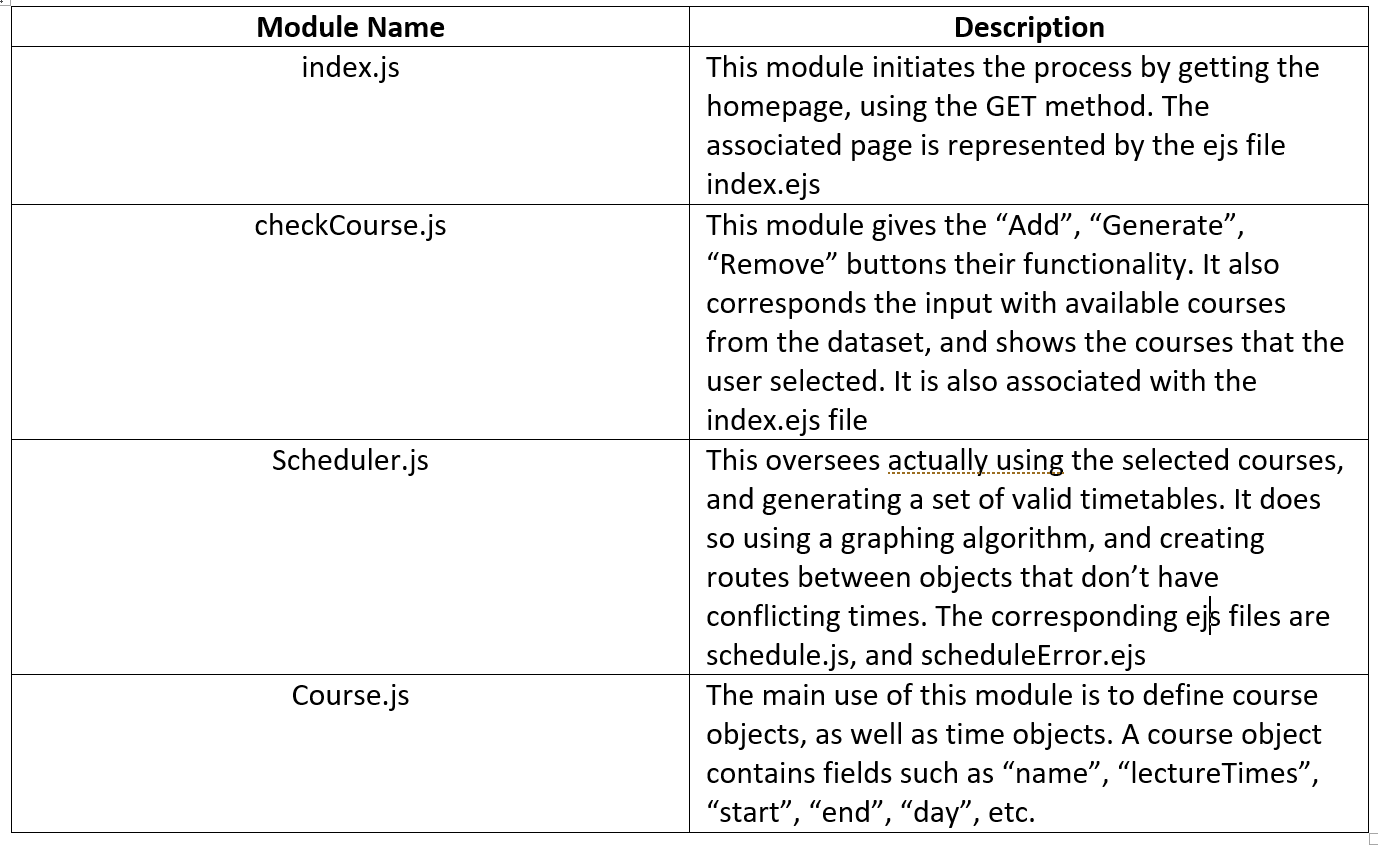
\includegraphics[width=5in]{images/Software_Description.png} 
   \caption{Software Description}
   \label{s_d}
\end{figure}


\subsection{Test Team}
The entire Genzter team will be in tasked with testing. Testing shall be evenly divided between members.

\subsection{Automated Testing Approach}
As stated above, automated testing will be done using the javascript testing framework called \href{http://mochajs.org}{Mocha}. Accompanying Mocha will be an assertion library called \href{http://chaijs.com/}{Chai}. Unit tests will be set up, and the framework will be used to automatically run through all the unit tests, and reveal any faults that may reside in the program. The unit tests will include normal input, boundary cases, as well as extreme cases and conflicting cases. This will ensure that the program functions expectedly, and that no special cases were missed. In other words, this automated testing approach will make sure that in any case, the program will have a path to follow, and its behaviour can be predicted.

\subsection{Testing Tools}
For unit testing we will be using the testing framework \href{http://mochajs.org}{Mocha}. System testing will be conducted on internet browsers. Code analysis will be done by the Genzter team.

\subsection{Testing Schedule}
The testing schedule is included in the Gantt chart, located in the Project Schedule folder in the main directory.

\newpage

\section{System Test Description}
\subsection{Tests for Functional Requirements}
\subsubsection{Test Area 1 \\ Conflict Detection Test}
\begin{enumerate}
\item Type: Dynamic \\
Initial State: Homepage \\
Input: SFWRENG 3RA3, EARTHSC 2EI3 \\
\textcolor{blue}{Expected Output: Conflict error page} \\
The courses in the input field will be selected and added in the UI manually. The expected result, an error page, will be checked against the actual output. The courses selected must have conflicting time slots. \\

\item Type: Dynamic \\
Initial State: Homepage \\
Input: RELIGST-2TA3, SFWRENG 3BB4 \\
\textcolor{blue}{Expected Output: Conflict error page} \\
The courses in the input field will be selected and added in the UI manually. The expected result, an error page, will be checked against the actual output. The courses selected must have conflicting time slots. \\


\item Type: Dynamic \\
Initial State: Homepage \\
Input: BIOLOGY 2F03, SFWRENG 3MX3 \\
\textcolor{blue}{Expected Output: Conflict error page} \\
The courses in the input field will be selected and added in the UI manually. The expected result, an error page, will be checked against the actual output. The courses selected must have conflicting time slots. \\


\item Type: Dynamic \\
Initial State: Homepage \\
Input: MATLS 2B03, EARTHSC 2EI3 \\
\textcolor{blue}{Expected Output: Conflict error page} \\
The courses in the input field will be selected and added in the UI manually. The expected result, an error page, will be checked against the actual output. The courses selected must have conflicting time slots. \\
\end{enumerate}

\subsubsection{Test Area 2: Output Timetable}
\begin{enumerate}
\item Type: Automated \\
Initial State: Homepage \\
Input: SFWRENG 3XA3, SFWRENG 3BB4, SFWRENG 3DB3, SFWRENG 3MX3, COMMERCE 1AA3 \\
\textcolor{blue}{Expected Output: Valid Schedule in a timetable format.} \\
The courses in the input field will be selected and added in the UI manually. The expected result, a color coded schedule, will be checked against the actual output. Generated timetable must have every core, tutorial, lab etc. required for each course. It will be manually checked against the dataset and our own timetables \\

\item Type: Automated \\
Initial State: Homepage \\
Input:  ENGINEER-1C03, MATH-1ZC3, MATH-1ZB3,  ECON-1BB3, PHYSICS-1E03, MATLS-1M03 \\
\textcolor{blue}{Expected Output: Valid Schedule in a timetable format.} \\
The courses in the input field will be selected and added in the UI manually. The expected result, a color coded schedule, will be checked against the actual output. Generated timetable must have every core, tutorial, lab etc. required for each course. It will be manually checked against the dataset and our own timetables \\

\item Type: Manual \\
Initial State: Homepage \\
Input: RELIGST-2TA3, RELIGST-2QQ3, POLSCI-2I03, POLSCI-4CA3\\
\textcolor{blue}{Expected Output: Valid Schedule in a timetable format.} \\
The courses in the input field will be selected and added in the UI manually. The expected result, a color coded schedule, will be checked against the actual Expected Output. Generated timetable must have every core, tutorial, lab etc. required for each course. It will be manually checked against the dataset and our own timetables \\

\item Type: Manual \\
Initial State: Homepage \\
Input:EARTHSC-2EI3, EARTHSC-2C03, GEOG-2UI3, GEOG-2GI3, BIOLOGY-2F03\\
\textcolor{blue}{Expected Output: Valid Schedule in a timetable format.} \\
The courses in the input field will be selected and added in the UI manually. The expected result, a color coded schedule, will be checked against the actual output. Generated timetable must have every core, tutorial, lab etc. required for each course. It will be manually checked against the dataset and our own timetables \\
\end{enumerate}

\subsubsection{Regression Testing}
Regression testing will continually happen to ensure all features continue to function ideally, no matter the changes occurring to the program.

\subsubsection{Parallel Testing}
Please refer to \hyperref[sec:compare]{this section}

\subsection{Tests for Non-functional Requirements}
\subsubsection{Test Area 3: Speed Performance}
\begin{enumerate}

\item Type: Manual \\
Initial State: Homepage \\
Input: SFWRENG 3XA3, SFWRENG 3BB4, SFWRENG 3DB3, SFWRENG 3MX3, COMMERCE 1AA3 \\
\textcolor{blue}{Expected Output: Output should be displayed within 3 seconds} \\
The input courses shall be selected, and the the generator is timed from when the "Generate" button is pressed. \\

\item Type: Manual \\
Initial State: Homepage \\
Input:  ENGINEER-1C03, MATH-1ZC3, MATH-1ZB3,  ECON-1BB3, PHYSICS-1E03, MATLS-1M03 \\
\textcolor{blue}{Expected Output: Output should be displayed within 3 seconds} \\
The input courses shall be selected, and the the generator is timed from when the "Generate" button is pressed.  \\
\end{enumerate}

\subsubsection{Test Area 4: UI}
\begin{enumerate}

\item Type: Manual \\
Initial State: Homepage \\
Input: Any McMaster Course \\
\textcolor{blue}{Expected Output: Add course to list of courses} \\
Any McMaster course is selected, and the "Add" button is pressed. This is to test the ability of the UI to retrieve input from the user. \\

\item Type: Manual \\
Initial State: Homepage with list of courses chosen\\
Input:  Pressing the "Remove" button \\
\textcolor{blue}{Expected Output: Removal of the selected course} \\
Starting off with a list of courses, the "Remove" button will be pressed to test the ability of the UI to modify the course list at the request of the user.  \\


\item Type: Manual \\
Initial State: Homepage with list of courses chosen\\
Input:  Pressing the "Generate" button \\
\textcolor{blue}{Expected Output: Timetable} \\
Starting off with a list of courses, the "Generate" button will be pressed to test the ability of the UI to display output at the request of the user.  \\
\end{enumerate}

\subsubsection{Test Area 5: Maintainability and Robustness}
\begin{enumerate}
\item Type: Static \\
Initial State: Not running \\
Input: Code walkthrough and inspection\\
\textcolor{blue}{Expected Output: N/A} \\
This test is a static test for confirming the syntax and structural integrity of the backend of the program.\\


\textcolor{blue}{
\item Type: Dynamic \\
Initial State: Homepage \\
Input: ENGINEER-1C03, MATH-1ZC3, MATH-1ZB3,  ECON-1BB3, PHYSICS-1E03, MATLS-1M03, ECON-1B03, MATH-1ZA3, ENGINEER-1D04, CHEM-1E03\\
Expected Output: Valid Schedule in a timetable format \\
Actual output: The result was a valid, working schedule with all necessary items
}
\end{enumerate}

\begin{enumerate}
\item \textcolor{blue}{Type: Static, Automated \\
Initial State: Not running \\
Input: Code inspected automatically by \href{http://jshint.com}{JSHint}} \\
\textcolor{blue}{Expected Output: N/A \\
This test is an automatic test for confirming the syntax and structural integrity of the backend of the program.}\\ 
\end{enumerate}

\textcolor{blue}{
\subsubsection{Test Area 6: Browser Compatability}}
\begin{enumerate}
\item \textcolor{blue}{Type: Static \\
Initial State: Not running \\
Input: Visit website using different browers\\}
\textcolor{blue}{Expected Output: N/A \\
This test is a static test for confirming that the website works for various browsers. } \\
\end{enumerate}

\subsubsection{Traceability}
\begin{table}[h]
\begin{center}
\begin{tabular}{ | c | c | c | c | c | c | }
\hline
 Requirement & TA1 & TA2 & TA3 & TA4 & TA5  \\ 
\hline
 2.7.1 & X & & & &   \\  
\hline
 2.7.2 & & X & X & X & \\
\hline 
 3.2 & & & & X & \\ 
\hline
 3.3 & & & X & & \\
\hline
 3.5 & & & & & X \\
\hline
\end{tabular}
\end{center}
\caption{Traceability Matrix}
\end{table}
\newpage

\section{PoC Test}

\subsection{Conflict Detection}
\begin{enumerate}
\item Type: Dynamic \\
Initial State: Homepage \\
Input: BIOLOGY 2F03, SFWRENG 3MX3 \\
\textcolor{blue}{Expected Output: Conflict error page} \\
The courses in the input field will be selected and added in the UI manually. The expected result, an error page, will be checked against the actual output. The courses selected must have conflicting time slots. \\
\end{enumerate}

\subsection{Schedule Output}
\begin{enumerate}
\item Type: Manual \\
Initial State: Homepage \\
Input: SFWRENG 3XA3, SFWRENG 3BB4 \\
\textcolor{blue}{Expected Output: Valid Schedule in a timetable format.} \\
The courses in the input field will be selected and added in the UI manually. The expected result, a color coded schedule, will be checked against the actual output. Generated timetable must have every core, tutorial, lab etc. required for each course. It will be manually checked against the dataset and our own timetables \\
\end{enumerate}

\section{Comparison to Existing Implementation}\label{sec:compare}
The project will be benchmarked against two existing implementations, \url{http://timetablegenerator.io} and \url{https://github.com/ash47/TimetableGenerator}. Mainly, we will be comparing our project with \url{http://timetablegenerator.io} because it uses the McMaster database as well, so we can fully compare the generated timetables. The outputs are fairly similar, so comparison should not be very difficult. The comparison will be done manually by the testing team.
\section{Unit Testing Plan}
Unit tests will be defined by specific modules and their functionality. So for example, from the software description figure, index will have a set of unit tests, and checkCourse will have its own, and so forth. Each module will have its own type of tests. We may need to implement stubs, to imitate connection to the database, to ensure the right functions are being called, etc. As for code coverage, equivalence will definitely be used throughout the majority of the test cases. Boundary cases will be used. An example of such a boundary case would be using a full year, six unit course as input, and testing the behaviour of the program. This is a boundary case because the program has had some trouble with full year courses. Lastly, control-flow testing will be implemented in order to extensively test as much lines of code as possible, and ensure that every path and edge is covered. As for specific details, that is still unclear at the moment, but will be updated and posted as soon as a defined  and detailed plan is created.
\end{document}
